%\documentclass[
  bibliography=totoc,     % Literatur im Inhaltsverzeichnis
  captions=tableheading,  % Tabellenüberschriften
  titlepage=firstiscover, % Titelseite ist Deckblatt
]{scrartcl}

% Paket float verbessern
\usepackage{scrhack}

% Warnung, falls nochmal kompiliert werden muss
\usepackage[aux]{rerunfilecheck}

% unverzichtbare Mathe-Befehle
\usepackage{amsmath}
% viele Mathe-Symbole
\usepackage{amssymb}
% Erweiterungen für amsmath
\usepackage{mathtools}

% Fonteinstellungen
\usepackage{fontspec}
% Latin Modern Fonts werden automatisch geladen
% Alternativ zum Beispiel:
%\setromanfont{Libertinus Serif}
%\setsansfont{Libertinus Sans}
%\setmonofont{Libertinus Mono}

% Wenn man andere Schriftarten gesetzt hat,
% sollte man das Seiten-Layout neu berechnen lassen
\recalctypearea{}

% deutsche Spracheinstellungen
\usepackage[ngerman]{babel}


\usepackage[
  math-style=ISO,    % ┐
  bold-style=ISO,    % │
  sans-style=italic, % │ ISO-Standard folgen
  nabla=upright,     % │
  partial=upright,   % │
  mathrm=sym,        % ┘
  warnings-off={           % ┐
    mathtools-colon,       % │ unnötige Warnungen ausschalten
    mathtools-overbracket, % │
  },                       % ┘
]{unicode-math}

% traditionelle Fonts für Mathematik
\setmathfont{Latin Modern Math}
% Alternativ zum Beispiel:
%\setmathfont{Libertinus Math}

\setmathfont{XITS Math}[range={scr, bfscr}]
\setmathfont{XITS Math}[range={cal, bfcal}, StylisticSet=1]

% Zahlen und Einheiten
\usepackage[
  locale=DE,                   % deutsche Einstellungen
  separate-uncertainty=true,   % immer Unsicherheit mit \pm
  per-mode=symbol-or-fraction, % / in inline math, fraction in display math
]{siunitx}

% chemische Formeln
\usepackage[
  version=4,
  math-greek=default, % ┐ mit unicode-math zusammenarbeiten
  text-greek=default, % ┘
]{mhchem}

% richtige Anführungszeichen
\usepackage[autostyle]{csquotes}

% schöne Brüche im Text
\usepackage{xfrac}

% Standardplatzierung für Floats einstellen
\usepackage{float}
\floatplacement{figure}{htbp}
\floatplacement{table}{htbp}

% Floats innerhalb einer Section halten
\usepackage[
  section, % Floats innerhalb der Section halten
  below,   % unterhalb der Section aber auf der selben Seite ist ok
]{placeins}

% Seite drehen für breite Tabellen: landscape Umgebung
\usepackage{pdflscape}

% Captions schöner machen.
\usepackage[
  labelfont=bf,        % Tabelle x: Abbildung y: ist jetzt fett
  font=small,          % Schrift etwas kleiner als Dokument
  width=0.9\textwidth, % maximale Breite einer Caption schmaler
]{caption}
% subfigure, subtable, subref
\usepackage{subcaption}

% Grafiken können eingebunden werden
\usepackage{graphicx}

% schöne Tabellen
\usepackage{tabularray}
\UseTblrLibrary{booktabs, siunitx}

% Verbesserungen am Schriftbild
\usepackage{microtype}

% Literaturverzeichnis
\usepackage[
  backend=biber,
]{biblatex}
% Quellendatenbank
\addbibresource{lit.bib}
\addbibresource{programme.bib}

% Hyperlinks im Dokument
\usepackage[
  german,
  unicode,        % Unicode in PDF-Attributen erlauben
  pdfusetitle,    % Titel, Autoren und Datum als PDF-Attribute
  pdfcreator={},  % ┐ PDF-Attribute säubern
  pdfproducer={}, % ┘
]{hyperref}
% erweiterte Bookmarks im PDF
\usepackage{bookmark}

% Trennung von Wörtern mit Strichen
\usepackage[shortcuts]{extdash}

\author{%
  Vincent Wirsdörfer\\%
  \href{mailto:vincent.wirsdoerfer@udo.edu}{authorA@udo.edu}%
  \and%
  Joris Daus\\%
  \href{mailto:joris.daus@udo.edu}{authorB@udo.edu}%
}
\publishers{TU Dortmund – Fakultät Physik}


%\begin{document}
\section{Auswertung}
\label{sec:Auswertung}

Zu Beginn soll der Dampfdruck $p_\text{sät}$ und die mittlere freie Weglänge $\bar {w}$ für die Temperaturen der Messreihen bestimmt werden.
Der Sättigungsdampfdruck wird über $ausfüllen$ und die mittlere freie Weglänge über $ausfüllen$ bestimmt. So ergeben sich die folgenden Werte

\begin{table}
    \centering
    \sisetup{ per-mode=reciprocal, table-format=2.2}
    \caption{Temperaturen, Drücke und mittlere freie Weglängen der verschiedenen Kurven.}
    \begin{tblr}{
        colspec = {S S S S S},
        row{1} = {guard, mode=math},
        }
        \toprule
        Kurve & 
        T \mathbin{/} \unit{\kelvin} &
        p_{sät} \mathbin{/} \unit{\milli \bar} &
        \bar w \mathbin{/} \unit{\centi \meter} & 
        \frac{a}{\bar w} \\
        \midrule
        \text{blau \ref{fig:Bremsspannung}} &   298.15  &   \num{0.0053}    &   \num{5.47e-01}  &   \num{1.83e+00}  \\  
        \text{rot \ref{fig:Bremsspannung}}  &   414.55  &   \num{3.44}      &   \num{8.42e-04}  &   \num{1.19e+03}  \\  
        \text{rot klein \ref{fig:Besch}}    &   438.15  &   \num{8.41}      &   \num{3.45e-04}  &   \num{2.90e+03}  \\  
        \text{rot groß \ref{fig:Besch}}     &   447.15  &   \num{11.5}      &   \num{2.51e-04}  &   \num{3.98e+03}  \\  
        \text{blau \ref{fig:Besch}}         &   459.15  &   \num{17.2}      &   \num{1.68e-04}  &   \num{5.95e+03}  \\ 
        \bottomrule
    \end{tblr}
    \label{tab:basics}
  \end{table}

\noindent Der Faktor $\frac{a}{w}$, wobei $a = \qty{1}{\centi\meter}$ bei der verwendeten Röhre beträgt, sollte einen Wert von $1000-4000$ besitzen. 
Dies ist immer außer bei der ersten und letzten Messung der Fall. Dies liegt an der vorherrschenden Temperatur.


\subsection{Integrale Energieverteilung der Elektronen}

Im Folgenden wird nun das Millimeterpapier ausgewertet. Dazu werden die markierten Stellen, an denen die Spannung notiert wird vermessen und 
zwischen denen der Bereich linear aufgeteilt. So kann sowohl die Spannung als auch der Strom über einen einfachen Dreisatz vermessen werden.
Dabei werden die Messpaare in einem Abstand von $\increment U_A =\qty{1}{\volt}$ vermessen. Die ausgewerteten Kurven sehen folgendermaßen aus.

\begin{figure}[H]
    \centering
    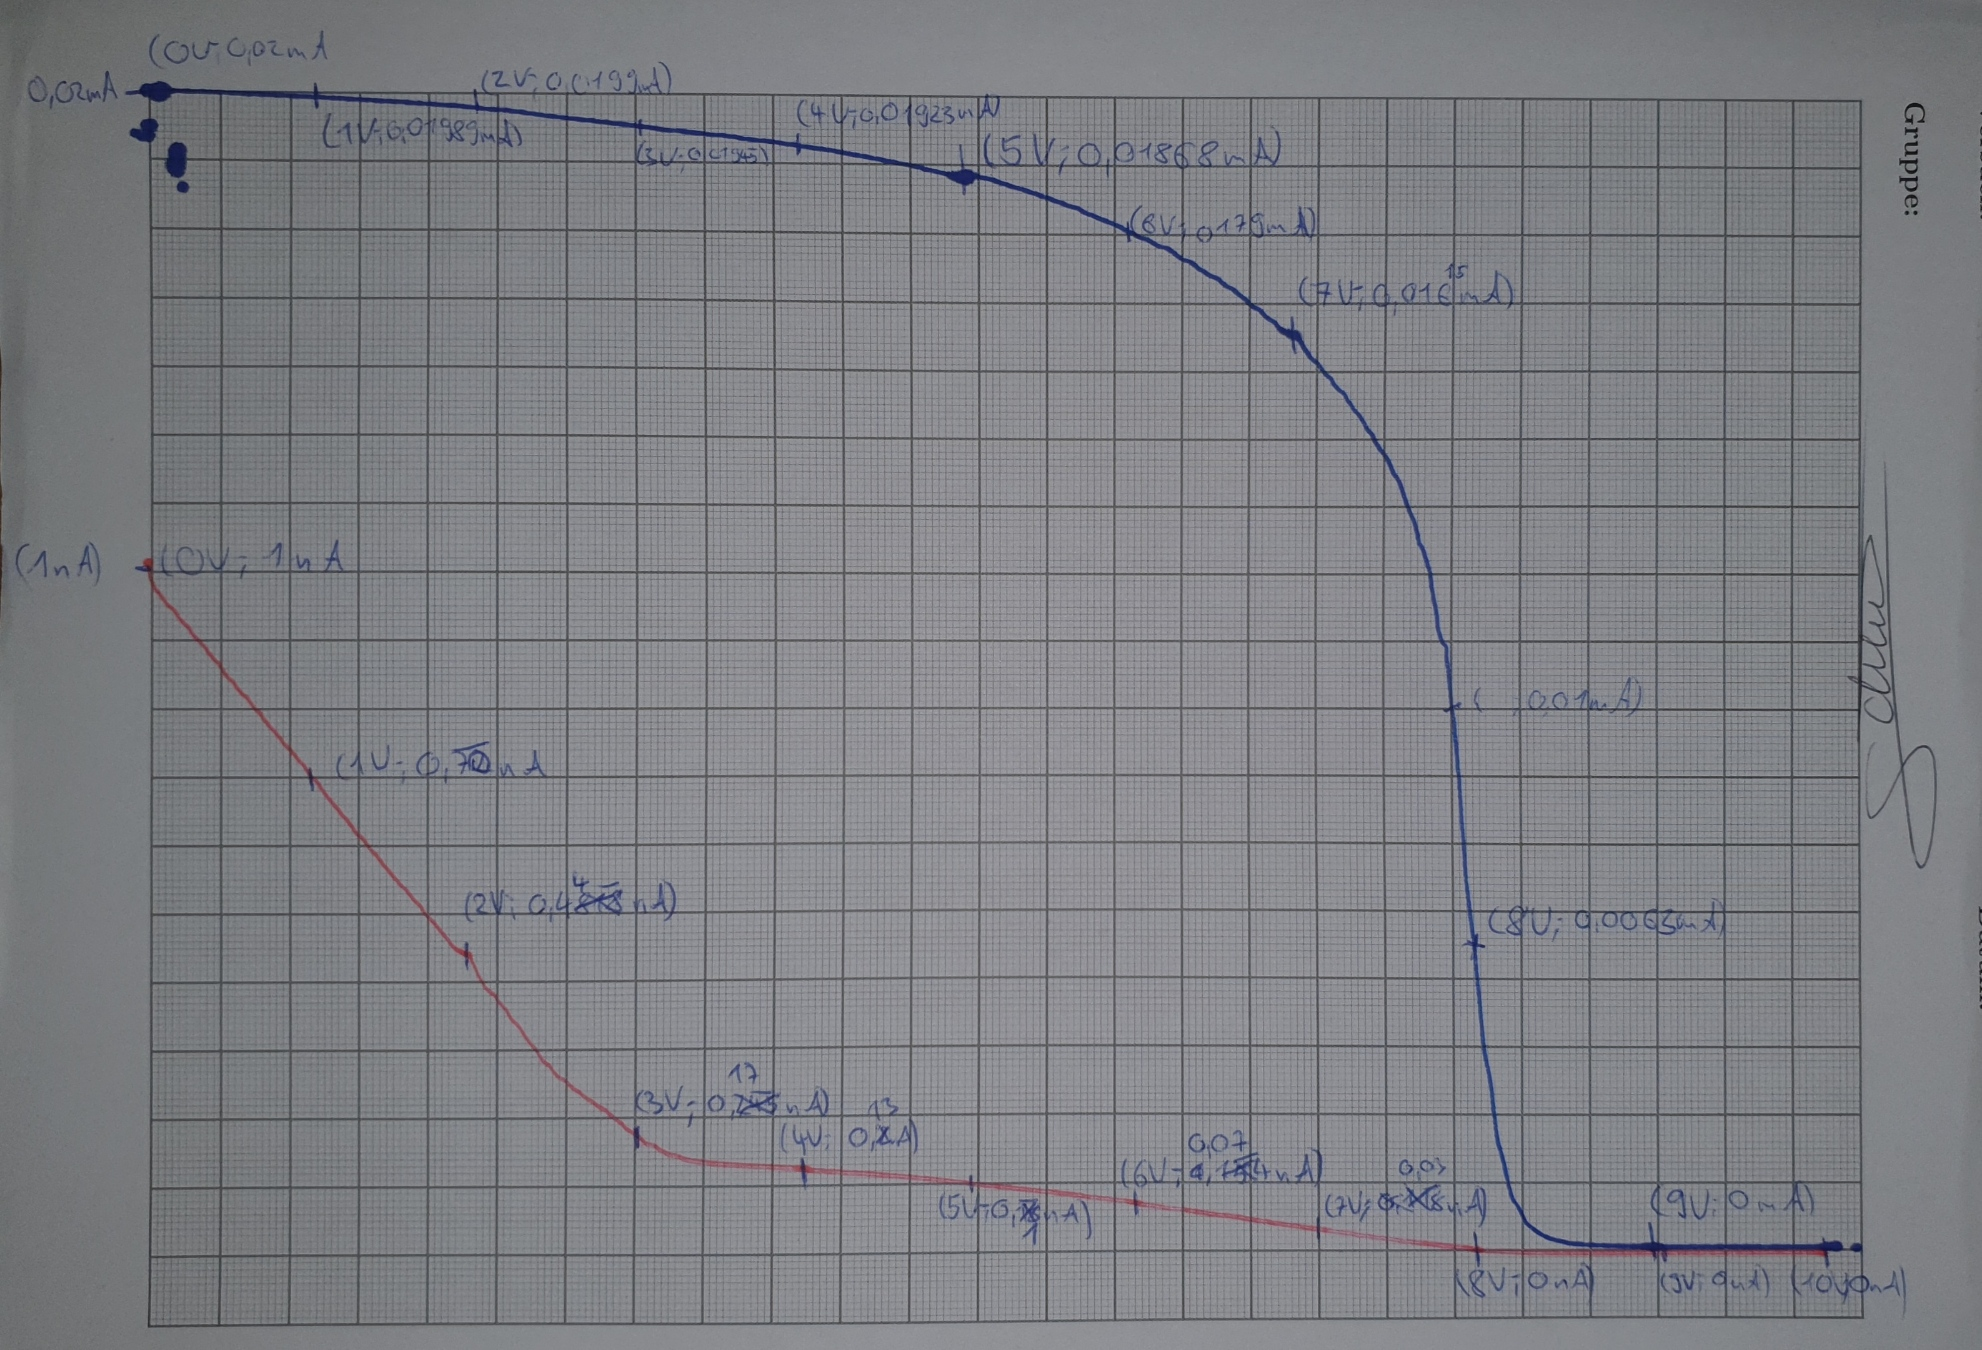
\includegraphics[width=0.9\textwidth]{content/Bremsspannung.jpg}
    \caption{Anodenstrom gegen Bremsspannung aufgetragen.}
    \label{fig:Bremsspannung}
\end{figure}

\noindent Anschließend wird jeweils die Differenz des Stroms $\increment I_A$ zum vorherigen Wert berechnet.
Auf diese Weise ergeben sich die folgenden Messwerte


\begin{table}[H]
    \caption{Differentielle Energieverteilung der Elektronen.}
    \begin{minipage}[t]{0.5\textwidth}
        \label{tab:blau25}
        \caption{blaue Kurve bei \qty{25}{\celsius}}
        \vspace{0pt}
        \centering
    \begin{tblr}{
        colspec = {S[table-format=1.2] S[table-format=1.3]},
        row{1} = {guard, mode = math},
        }
        \toprule
        U_A \mathbin{/} \unit{\volt} & \increment I_A \mathbin{/} \unit{\milli\ampere} \\
        \midrule
        1   &   0,00011     \\
        2   &   -0,00001    \\
        3   &   0,00045     \\
        4   &   0,00022     \\
        5   &   0,00055     \\
        6   &   0,00078     \\
        7   &   0,0019      \\
        8   &   0,0097      \\
        9   &   0,0063      \\
        10  &   0           \\ 
    \end{tblr}
\end{minipage} \hfill
\begin{minipage}[t]{0.5\textwidth}
        \vspace{0pt}
        \centering
        \caption{rote Kurve bei \qty{141,4}{\celsius}}
    \begin{tblr}{
            colspec={S[table-format=1.2] S[table-format=1.3]},
            row{1} = {guard, mode = math},
        }
        \toprule
        U_A  \mathbin{/} \unit{\volt} & \increment I_A \mathbin{/} \unit{\nano\ampere} \\
        \midrule
        1   &   0,30    \\
        2   &   0,26    \\
        3   &   0,27    \\
        4   &   0,04    \\
        5   &   0,03    \\
        6   &   0,03    \\
        7   &   0,04    \\
        8   &   0,03    \\
        9   &   0,00    \\
        10  &   0,00    \\
        \end{tblr}
    \end{minipage}\hfill
\end{table}

\noindent Diese Ableitungen \footnote{Die Differenz entspricht hier der Ableitung, da eine Schrittweite von \qty{1}{\volt} gewählt wurde.} 
können nun aufgetragen werden zur besseren Visualisierung. So entsteht der folgende Plot

\begin{figure}[H]
    \centering
    \includegraphics[width=0.9\textwidth]{Steigung.pdf}
    \caption{Differenz der Ströme aufgetragen gegen die Bremsspannung.}
\end{figure}

\noindent Die blaue Kurve besitzt einen starken Abfall, da es einen Häufungswert für die Energie von Elektronen gibt. Dieser 
ist das Maximum der Ableitung der Verteilung.
Zu sehen ist hier, dass die meisten Elektronen eine Energie um \qty{8}{\electronvolt} besitzen, da der maximale Anodenstrom 
bei \qty{8}{\volt} liegt. So ergibt sich 
bei \qty{25}{\celsius} ein Kontaktpotential von 

\begin{align*}
    K=U_B - U_{A; max} = \qty{9}{\volt} - \qty{8}{\volt} = \qty{1.5}{\volt}
\end{align*}


\subsection{Die Franck-Hertz Kurve}
Für die Auswertung der Franck-Hertz Kurve wird die obere rote Kurve aus \ref{fig:Besch} verwendet. Diese wird bei \qty{447.15}{\kelvin} 
aufgenommen. Es wurden Markierungen bei \qty{10}{\volt}, \qty{20}{\volt} und \qty{30}{\volt} gesetzt. So können die Zwischenschritte 
mit einem Dreisatz gelegt werden und die Spannung der Maxima vermessen werden. Es werden anschließend wieder die Differenzen berechnet. 
Die ausgewertete Kurve sieht folgendermaßen aus.

\begin{figure}[H]
    \centering
    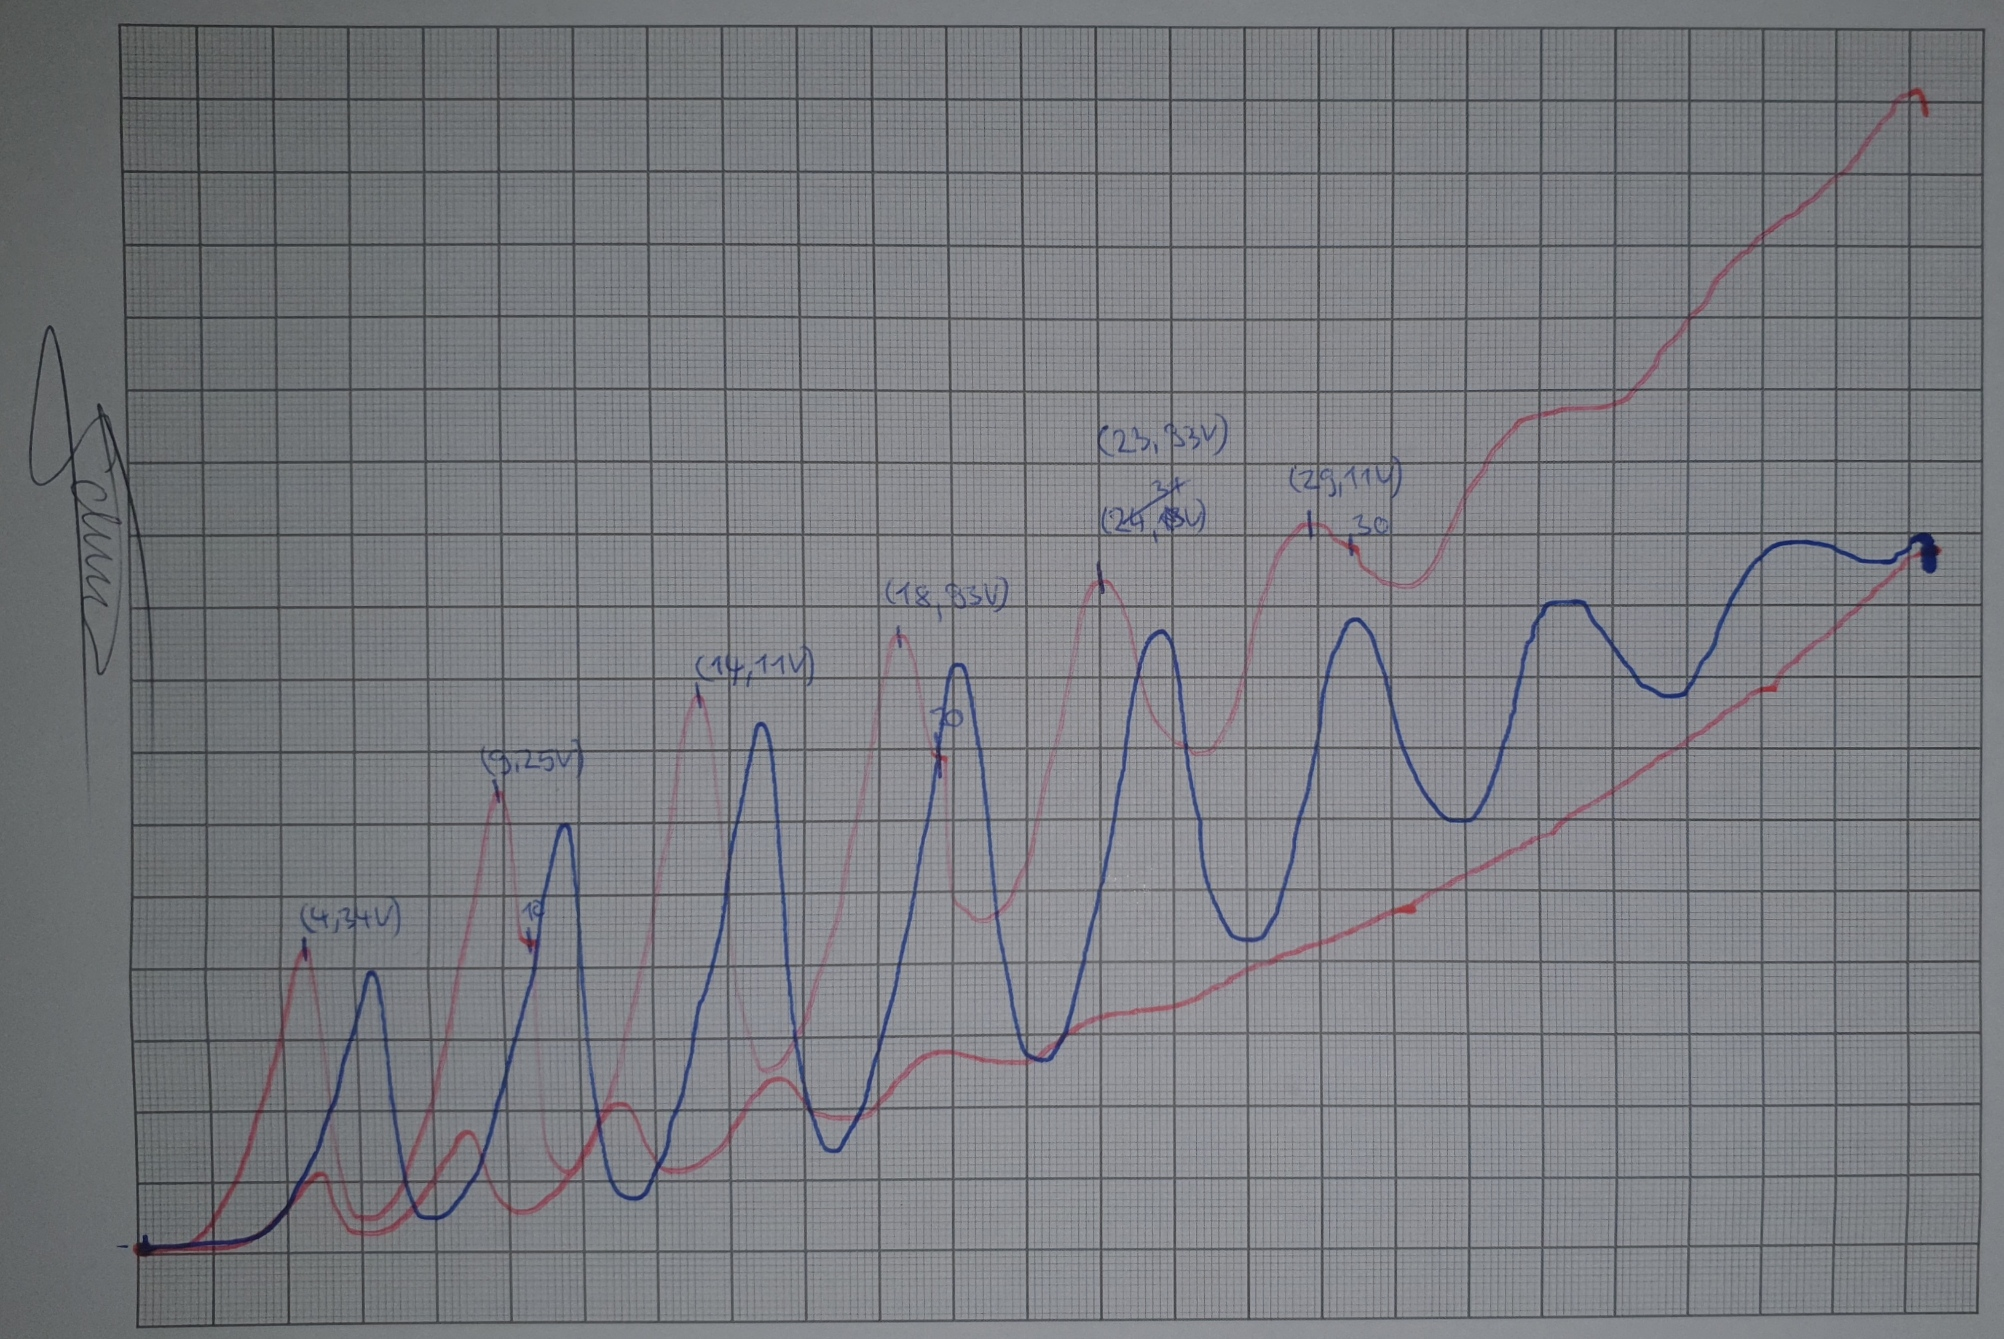
\includegraphics[width=0.9\textwidth]{content/FranckHertz.jpg}
    \caption{Anodenstrom gegen Beschleunigungsspannung aufgetragen.}
    \label{fig:Besch}
\end{figure}

So ergeben sich die folgenden Werte:


\begin{table}[H]
    \caption{Maxima und deren Abstände der Franck-Hertz Kurve.}
        \label{tab:blau25}
        \centering
    \begin{tblr}{
        colspec = {S[table-format=2.2] S[table-format=1.2]},
        row{1} = {guard, mode = math},
        }
        \toprule
        U_B \mathbin{/} \unit{\volt} & \increment U_B \mathbin{/} \unit{\volt} \\
        \midrule
        4.34    &   /       \\
        9.25    &   4.91    \\
        14.11   &   4.86    \\
        18.93   &   4.82    \\
        23.93   &   5.00    \\
        29.11   &   5.18    \\        
    \end{tblr}
\end{table}

\noindent Es wird nun der Mittelwert von den Differenzen gebildet, um eine durchschnittliche Energieänderung zu erhalten. Diese ergibt 
sich zu 

\begin{align}
    \bar U_{b\text{, max}} = \qty{4.95\pm0.13}{\volt}
    \label{eqn:meanU}
\end{align}

\noindent Mit dieser mittleren Energie kann nun die Wellenlänge berechnet werden, welche das Hg-Atom nach der Anregung abstrahlt. 
Dazu werden die Energien $E=hf=eU$ nach $f$ aufgelöst und in $\lambda = \frac{c}{f}$ eingesetzt. So ergibt sich 

\begin{equation*}
    \lambda = \frac{h c}{e U_{b\text{, max}}} = \qty{250\pm6}{\nano\meter}
\end{equation*}


















%\end{document}
